% Shared standalone design for the editable figure reconstructions.
\documentclass[tikz,border=5pt,10pt]{standalone}
\usepackage[T1]{fontenc}
\usepackage[utf8]{inputenc}
\usepackage{newpxtext,newpxmath}
\usepackage[scaled=.94]{sourcesanspro}
\usepackage{pgfplots}
\pgfplotsset{compat=1.18}
\usetikzlibrary{arrows.meta,calc,positioning,decorations.pathreplacing,
  decorations.markings,patterns,matrix,shapes.geometric,fit,backgrounds,
  intersections,angles,quotes}
\definecolor{ink}{HTML}{203746}
\definecolor{accent}{HTML}{146C78}
\definecolor{muted}{HTML}{667780}
\definecolor{signalred}{HTML}{B94B44}
\color{ink}
\tikzset{>=Latex,line width=.8pt,
  every node/.style={font=\small},
  axis/.style={->,draw=muted,line width=.5pt},
  guide/.style={draw=muted,dashed,line width=.45pt},
  curve/.style={draw=accent,line width=1pt},
  marker/.style={circle,fill=accent,inner sep=1.5pt},
  labelbox/.style={fill=white,inner sep=2pt}}

\begin{document}
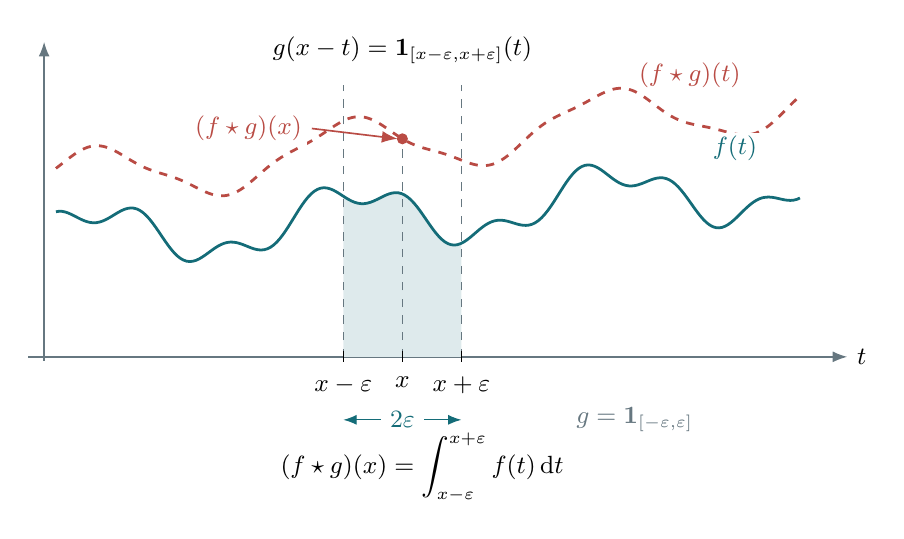
\begin{tikzpicture}[x=1cm,y=1cm]
% The box has width 2 epsilon = 1.5; it is not normalized to unit mass.
% Integrating each sinusoid gives exactly 2 sin(k epsilon)/k times sin(k t).
\pgfmathdeclarefunction{signal}{1}{\pgfmathparse{1.45+.075*#1+.35*sin(110*#1)+.16*sin(320*#1)}}
\pgfmathdeclarefunction{smoothed}{1}{\pgfmathparse{1.5*(1.45+.075*#1)+.70*sin(82.5)/(110*pi/180)*sin(110*#1)+.32*sin(240)/(320*pi/180)*sin(320*#1)}}
\draw[axis] (0,0)--(10.4,0) node[right] {$t$};
\draw[axis] (.2,-.05)--(.2,4.0);
\fill[accent!14] plot[domain=4:5.5,samples=70] (\x,{signal(\x)}) -- (5.5,0)--(4,0)--cycle;
\draw[curve,domain=.35:9.8,samples=240] plot (\x,{signal(\x)});
\draw[signalred,dashed,line width=1pt,domain=.35:9.8,samples=240] plot (\x,{smoothed(\x)});
\draw[guide] (4,0)--(4,3.45) (5.5,0)--(5.5,3.45);
\node[anchor=south] at (4.75,3.6) {$g(x-t)=\mathbf{1}_{[x-\varepsilon,x+\varepsilon]}(t)$};
\node[accent,fill=white,inner sep=1pt,anchor=west] at (8.65,2.65) {$f(t)$};
\node[signalred,fill=white,inner sep=1pt,anchor=south] at (8.4,3.38) {$(f\star g)(t)$};
\pgfmathsetmacro{\valueatx}{smoothed(4.75)}
\draw[guide] (4.75,0)--(4.75,\valueatx);
\fill[signalred] (4.75,\valueatx) circle(2pt);
\node[signalred,anchor=east,fill=white,inner sep=2pt] at (3.55,2.9) {$(f\star g)(x)$};
\draw[signalred,->,line width=.6pt] (3.6,2.9)--(4.69,\valueatx);
\foreach \x/\lab in {4/{x-\varepsilon},4.75/{x},5.5/{x+\varepsilon}} {
 \draw (\x,.07)--(\x,-.07); \node[below] at (\x,-.13) {$\lab$};}
\draw[<->,accent] (4,-.8)--node[fill=white] {$2\varepsilon$}(5.5,-.8);
\node[muted] at (7.7,-.8) {$g=\mathbf{1}_{[-\varepsilon,\varepsilon]}$};
\node at (5,-1.4) {$(f\star g)(x)=\displaystyle\int_{x-\varepsilon}^{x+\varepsilon}f(t)\,\mathrm{d}t$};
\end{tikzpicture}
\end{document}
